%%%%%%%%%%%%%%%%%%%%%%%%%%%%%%%%%%%%%%%%%%%%%%%%%%%%%%%%%%%%%%%%%%%%%%%%%%%
%
% Plantilla para un art�culo en LaTeX en espa�ol.
%
%%%%%%%%%%%%%%%%%%%%%%%%%%%%%%%%%%%%%%%%%%%%%%%%%%%%%%%%%%%%%%%%%%%%%%%%%%%

\documentclass{article}


% Esto es para poder escribir acentos directamente:
\usepackage[latin1]{inputenc}
% Esto es para que el LaTeX sepa que el texto est� en espa�ol:
\usepackage[spanish]{babel}
% Esto es para que se pueda crear el indice
\usepackage{makeidx}
% Paquetes de la AMS:
\usepackage{amsmath, amsthm, amsfonts}
% para poder poner una hoja apaisada
\usepackage{lscape}
%para incluir graficos
\usepackage{graphicx}
%para permitir que la imagen este donde yo quiero y no en otro lugar
\usepackage{float}
% para hipertexto
\usepackage{url}
% para poder envolver imagenes con texto
\usepackage{wrapfig}
%para los apendices
\usepackage[titletoc]{appendix}
% Esto es para poder modificar las dimensiones del texto
\usepackage{geometry}
\geometry{a4paper}

% Paquetes de la AMS:
\usepackage{amsmath, amsthm, amsfonts}

\graphicspath{ {Imagenes/} }

% Teoremas
%--------------------------------------------------------------------------
\newtheorem{thm}{Teorema}[section]
\newtheorem{cor}[thm]{Corolario}
\newtheorem{lem}[thm]{Lema}
\newtheorem{prop}[thm]{Proposici�n}
\theoremstyle{definition}
\newtheorem{defn}[thm]{Definici�n}
\theoremstyle{remark}
\newtheorem{rem}[thm]{Observaci�n}

% Atajos.
% Se pueden definir comandos nuevos para acortar cosas que se usan
% frecuentemente. Como ejemplo, aqu� se definen la R y la Z dobles que
% suelen representar a los conjuntos de n�meros reales y enteros.
%--------------------------------------------------------------------------

\def\RR{\mathbb{R}}
\def\ZZ{\mathbb{Z}}

% De la misma forma se pueden definir comandos con argumentos. Por
% ejemplo, aqu� definimos un comando para escribir el valor absoluto
% de algo m�s f�cilmente.
%--------------------------------------------------------------------------
\newcommand{\abs}[1]{\left\vert#1\right\vert}

% Operadores.
% Los operadores nuevos deben definirse como tales para que aparezcan
% correctamente. Como ejemplo definimos en jacobiano:
%--------------------------------------------------------------------------
\DeclareMathOperator{\Jac}{Jac}

%--------------------------------------------------------------------------
\title{\underline{Practica Profesional Supervisada} \\
\large \underline{Informe de las 100 horas} \\
\huge \textbf{ \\ Plataforma concentradora de sensores y eventos digitales} \\ }
\author{Autores: Ignacio Sambataro, Luciano Mantovani\\ \\
  \large Tutor: PhD. Ing. Orlando Micolini \\
  \large Supervisor: Ing. Maximiliano Eschoyez \\ \\
  \small Laboratorio de Arquitectura de Computadoras\\
  \small Facultad de Ciencias Exactas, Fisicas y Naturales\\
  \small Universidad Nacional de Cordoba\\
  \date{A�o 2015}
}


\makeindex
\begin{document}
\maketitle

%resumen
\abstract{Este informe contiene un resumen de las actividades realizadas para la practica profesional
supervisada en las primeras 100 horas de trabajo. El proyecto a realizar es una plataforma concentradora
de sensores y eventos digitales}

%salto de pagina
\clearpage



\section{Introducci�n}
Esta practica esta orientada al dise�o y la construccion de un sistema embebido que concentre las se�ales de varios sensores y varias fuentes de eventos digitales. La idea es que un sistema embebido de uso especifico pueda tercerizar la tarea de obtener, convertir y procesar una se�al de uno o varios sensor o una o varias fuente de eventos digitales.

Surgio de la problematica de algunos proyectos dentro del Laboratorio de Arquitectura de Computadoras que compartian el mismo problema. La necesidad de un sistema que genericamente obtenga las se�ales de los sensores y la pueda transmitir al sistema principal, ya convertidas. Ademas de un contador de eventos que no requiera del uso de interrupciones por software.

En este informe cubrimos los avances hechos en las primeras 100 horas de trabajo en el proyecto.


\section{Requerimientos}
\subsection{Principales}
\begin{itemize}
  \item Leer de 4 a 8 se�ales anal�gicas y convertirlas a digital.
  \item Contar eventos con 3 o 4 contadores distintos.
  \item Transmitir los datos digitales a trav�s de un protocolo serial a alguna otra placa o procesador.
\end{itemize}


\subsection{Secundarios}
\begin{itemize}
  \item Lograr el menor consumo posible.
  \item Buscar la mejor inmunidad al ruido, con una distancia de la placa a los sensores de hasta un m�ximo de 10 metros.
  \item Lograr un producto lo m�s peque�o posible.
  \item Lograr un producto programable
\end{itemize}

\section{Investigacion}
La etapa de investigacion consistio en encontrar un microcontrolador que satisfaga la mayor cantidad de requerimientos principales. El sistema entero consiste en interactuar con el nucleo, que es el microcontrolador, por lo que esta etapa requierio de analisis detallado de las opciones con las se contaba. En el cuadro\ref{tabla_micros} se pueden ver los microcontroladores considerados en la etapa de seleccion.

% Table generated by Excel2LaTeX from sheet 'Sheet1'
\clearpage

\begin{landscape} % TABLA DE MICROS

\begin{table}[!]
\centering
\begin{flushleft}
% Table generated by Excel2LaTeX from sheet 'Sheet1'
\scalebox{0.7}{
\begin{tabular}{|c|c|c|c|c|c|c|c|c|c|c|c|c|}
\hline
Fabricante & Modelo & RAM(K) & canales ADC & Referencia & Resolucion & ganancia & Contadores & low power & puerto serie & Dimension (') &   Pins &   Us\$ \\
\hline
 Intel & 8XC51GB &    256 &      8 &    GND & 8 bits &     no & 3 (16 bits) &     si & salida y entrada RS232 &      N &     32 &      N \\
\hline
Silicon Labs & C8051F352 &    768 &      8 & DIF/GND & 24 bits &   128x & 4 (16 bits) &     si & Smbus/$I^{2}$C, UART, SPI & 0,35x0,35 &     32 &    2,3 \\
\hline
 Atmel & AT89C5115 &    256 &      8 &    GND & 8/10 bits &     no & 3 (16 bits) &     si & UART (3 modos Full Duplex) & 0,34x0,34 &     32 &     10 \\
\hline
Microchip & PIC18F4550 &     32 &     13 &    GND & 10 bits &     no & 4(8 y 16 bits) &     si & SPI, $I^{2}$C, UART/USART, USB & 0,47x0,47 &     44 &   5,36 \\
\hline
   Nec & PD78C17 &   1024 &      8 &    GND & 8 bits &     no & 2 (8 bits) &     si & Msbus/$I^{2}$C & 0,92x0,70 &     64 &      N \\
\hline
 Maxim & DS4830 & 1024x16 &     16 & DIF/GND & 13 bits &     no & 2(16 bits) &     si & SPI, $I^{2}$C & 0,2x0,2 &     40 &    7,5 \\
\hline
   NXP & LPC1110 &      4 &      8 &    GND & 10 bits &     no & 2(32 bits) &     si & $I^{2}$C, UART, Soporte RS-485 & 0,42x0,51 &     20 &    2,5 \\
\hline
 Atmel & ATSAM3A8C &    256 &     16 & DIF/GND & 12 bits &     no & 9(32 bits) &     si & USB, SPI & 0,63x0,63 &     63 &    2,4 \\
\hline
 Atmel & ATSAM3S1A &     64 &      8 & DIF/GND & 10/12 bits & 1x,2x,4x & 3(16 bits) &     si & USB, $I^{2}$C, SPI & 0,35x0,35 &     44 &    2,5 \\
\hline
 Atmel & ATSAM3S1C &     16 &     16 & DIF/GND & 10/12 bits & 1x,2x,4x & 6(16 bits) &     si & USB, $I^{2}$C, SPI & 0,63x0,63 &     74 &    2,5 \\
\hline
 Atmel & ATSAMD21J &    256 &     20 & DIF/GND & 12 bits &    16x & 5 (16 bits) &     si & 1 USB 2.0 + 6 $I^{2}$C/USART/SPI & 0,47x0,47 &     64 &      3 \\
\hline
 Atmel & ATSAMD21G &    256 &     14 & DIF/GND & 12 bits &    16x & 3 (16 bits) &     si & 1 USB 2.0 + 6 $I^{2}$C/USART/SPI & 0,35x0,35 &     48 &    2,5 \\
\hline
 Atmel & ATSAMD21E &    256 &     10 & DIF/GND & 12 bits &    16x & 3 (16 bits) &     si & 1 USB 2.0 + 4 $I^{2}$C/USART/SPI & 0,35x0,35 &     32 &    2,5 \\
\hline
Texas Instr & MSP430F5340 &     64 &      9 &    GND & 12 bits &     2x & 7 (distintas) &     si & SPI, $I^{2}$C, UART & 0,3x0,3 &     48 &    3,3 \\
\hline
    ST & STM32F373CX &    256 &      4 &    GND & 12, 16 bits &    32x & 17 (distintas) &     si & 2 $I^{2}$C, 3 SIP, 3 USART, 1 USB & 0,35x0,35 &     48 &    2,5 \\
\hline
Atmel AVR & ATmega128 &    128 & 8 (2 c/gain) & 7 DIF, 8 GND & 10 bits & 1x, 10x, 200x & 4 (8 y 16) &     si & USART, SPI & 0,6x0,6 &     64 &      8 \\
\hline
\end{tabular}



}
\end{flushleft}
  \caption{Microcontroladores considerados}\label{tabla_micros}
\end{table}

\end{landscape}

\subsection{Parametros tenidos en cuenta en la seleccion del microcontrolador}
\begin{itemize}
  \item \textbf{RAM:} No es un requisito principal, pero en caso de tener que decidir entre dos micros similares, el tama�o de la memoria puede ser un factor para tomar la decision final
  \item \textbf{Cantidad de canales del ADC:} Mientras mas canales se tengan, mas se�ales analogicas de entrada pueden haber, y mas se�ales de sensores se podran procesar simultaneamente
  \item \textbf{Referencia:} Nos dice si los pines del ADC se pueden usar como entrada diferencial o unicamente con referencia a GND. Esto es porque en el caso que haya 16 pines para el ADC y puedan usarse todos como entrada diferencial, se podrann usar como maximo la mitad de los pines, es decir 8.
  \item \textbf{Resolucion:} Es la cantidad de bits con la que se representa el dato convertido. A mayor resolucion, mayor presicion de la conversion.
  \item \textbf{Ganancia:} Una buena ganancia interna en el micro es necesaria para una amplificacion de la se�al.  evitando la mayor cantidad de ruido posible. Este parametro es clave si se quiere trabajar con sensores que funcionan a voltajes muy peque�os en ambientes susceptibles al ruido electrico.
  \item \textbf{Contadores:} Cantidad de timers en el microcontrolador que se utilizarian como contadores de eventos(es necesario que puedan ser clockeados por fuente externa, es decir, que la fuente que incrementa el contador provenga de eventos externos y no interiores al microcontrolador).
  \item \textbf{Modos de bajo consumo:} Si tiene mas de un modo de bajo consumo, es mas simple lograr que el sistema se encuentre el mayor tiempo posible consumiendo lo menor posible.
  \item \textbf{Puerto serie:} Interfaces seriales que soporta el micro. Minimamente se necesita que soporten $I^{2}$C y UART.
  \item \textbf{Dimension:} Dimension del micro. El tama�o de la placa deberia ser lo menor posible por lo que mientras mas peque�o el micro, mejor.
  \item \textbf{Cantidad de pines:} Dependiendo del encapsulado, habra una cantidad de pines. La cantidad puede afectar el tama�o y la complejidad de la placa.
  \item \textbf{Precio:} Costo en dolares del integrado.
\end{itemize}

\subsection{Selecci�n}
En el momento, habia en el laboratorio una placa de desarrollo de Silicon Labs con el microcontrolador C8051F352. Este mismo fue considerado dentro de las elecciones posibles, como puede verse en el cuadro \ref{tabla_micros}.

Ademas de la ventaja de tenerlo en el mismo laboratorio, la placa de Silicon Labs tiene la particularidad de tener una buena ganancia maxima (128x) a la entrada del ADC, lo cual lo distingue del resto de los microcontroladores analizados. Ademas de esto, cumple con el resto de los requisitos propuestos por nuestro tutor, por lo que consistia en una buena eleccion.

Habiendo hecho este analisis, se decidio optar por utilizar el microcontrolador C8051F352 de Silicon Labs.






\section{Silicon Labs \emph{C8051F352}}
En esta seccion se explicaran brevemente las funcionalidades que se utilizaron del microcontrolador elegido. Para informacion mas detallada referirse al datasheet del microcontrolador. \cite{bib:datasheet}

\subsection{Conversor Analogico-Digital}\label{sec:adc}
El C8051F350 incluye un ADC Sigma-Delta completamente diferencial de 16 bits con capacidad de calibracion interna, con capacidad de 8 mediciones simultaneas en modo singular, y 4 mediciones simultaneas en modo diferencial. Tiene dos filtros separados de decimacion programables con un throughput de hasta 1KHz. Tiene un voltaje de referencia interno de 2.5 V, y admite la administracion de voltajes de referencia externos. Cada canal puede ser amplificado 1, 2, 4, 8, 16, 32, 64, o 128 veces.

\subsubsection{Modos de medicion}
\begin{itemize}
  \item \textbf{Singular}: Entrada independiente medida con respecto a GND.
  \item \textbf{Diferencial}: Dos entradas medidas con respecto una de otra.
\end{itemize}

\subsubsection{Modos de conversion}
\begin{itemize}
  \item \textbf{Singular}: Indica al ADC que genere informacion suficiente para producir un resultado luego de un ciclo de conversion. El filtro puede ser \emph{fast-filter} o \emph{SINC3}. En el primero, el resultado esta disponible luego de un solo ciclo de conversion del ADC. En el segundo, espera 3 ciclos antes de que este disponible el resultado.
  \item \textbf{Continua}: El ADC comienza una nueva conversion inmediatamente despues de terminar la anterior. Los filtros funcionan de manera analoga al modo singular.
\end{itemize}

\subsection{Contadores}\label{sec:contadores}
El C8051F350 cuenta con 4 contadores: Timer0, Timer1, Timer2 y Timer3. Timer0 y Timer1 cuentan con 3 modos de operacion:
\begin{itemize}
  \item Contador de 13 bits
  \item Contador de 16 bits
  \item Contador de 8 bits con valor de retorno
\end{itemize}
Timer0 cuenta con un modo mas que es el de separarse en dos contadores independientes de 8 bits.
Timer2 y Timer3 tienen 2 modos:
 \begin{itemize}
   \item Contador de 16 bits con valor de retorno
   \item Dos contadores independientes de 8 bits con valor de retorno
 \end{itemize}

Todos los timers pueden ser clockeados por fuente interna o externa. En el caso de los timers 2 y 3 la fuente externa se divide por 8.

\subsection{Interfaz Serial}\label{sec:serial}
El C8051F352 cuenta con dos protocolos de transferencia serial de datos: SMBus y UART. \textbf{SMBus} es una interfaz de dos cables bi-direccional. Es compatible con $I^{2}$C, es por esto que se considera que este microcontrolador cuenta con $I^{2}$C por el hecho de tener SMBus. \textbf{UART} es una interfaz serial asincrona full-duplex.

\subsection{Flash}
Incluye una memoria Flash de 8 Kilobytes reprogramable dentro del chip para almacenamiento de datos no volatil. Es programable mediante interfaz C2 o por software

\section{Dise�o}

Luego de la eleccion de un microcontrolador, se inicio el proceso de dise�o. las figuras , , , muestran los diagramas que describen el sistema segun los requerimientos.

\subsection{Descripcion grafica del sistema}
\subsubsection{Diagrama de bloques}
\begin{figure}[h]
  \centering
  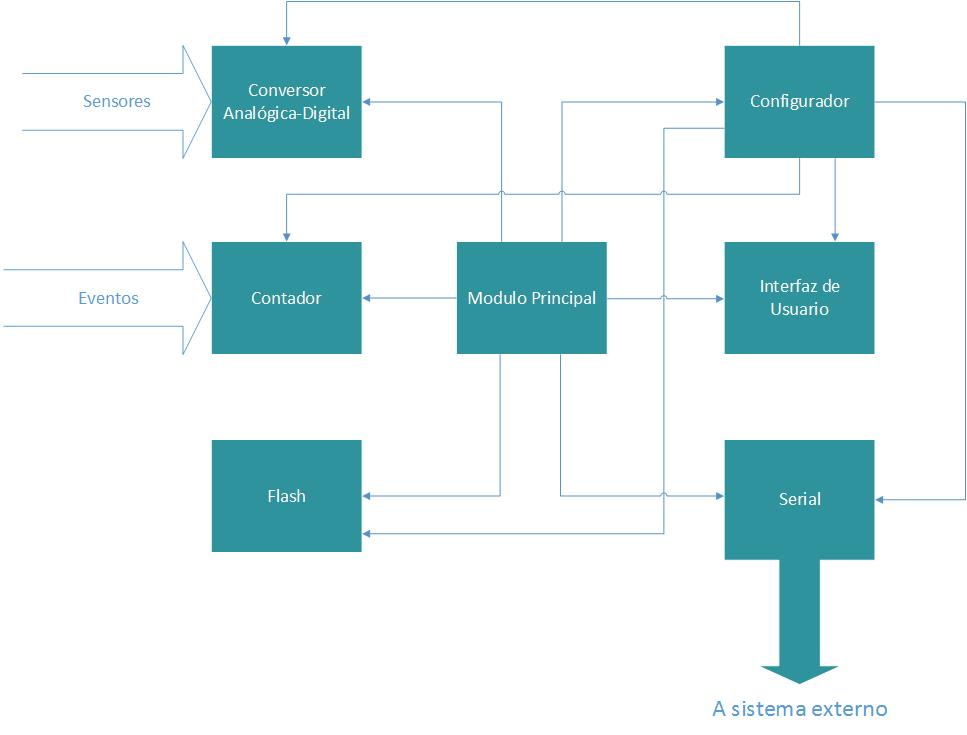
\includegraphics[width=0.80\textwidth, height = 9cm]{Bloques1}
  \caption{Diagrama de Bloques 1}\label{fig:bloques1}
\end{figure}

\paragraph{}
El sistema esta compuesto por 7 bloques o modulos separados, manejados por un modulo principal. En la figura \ref{fig:bloques1} se pueden observar estos bloques y la interaccion que tienen entre si.
\paragraph{}


\begin{itemize}
  \item El \textbf{Bloque Principal} se encarga ejecutar las funciones del resto de los modulos para dar arranque y ejecucion al sistema.
  \item El \textbf{Bloque Conversor Anal�gco-Digital} principalmente obtiene los datos de los sensores, los procesa, y los envia al modulo principal. Ademas de esto, configura el funcionamiento del ADC segun los parametros dados por el usuario. El usuario puede elegir la cantidad de pines que va a utilizar como entrada segun la cantidad de sensores que quiera medir, puede elegir un nivel de ganancia de amplificacion de la se�al antes de la conversion, y puede tambien elegir el modo de obtencion de los datos (diferencial o single-ended).
  \item El \textbf{Bloque Contador} se encarga de obtener los valores en los contadores de eventos.
  \item El \textbf{Bloque de Interfaz de Usuario} en este modulo se levanta la interfaz con la que interactua el usuario para establecer los parametros configurables del sistema.
  \item El \textbf{Bloque Configurador} interactua directamente con el hardware del microcontrolador. Realiza todas las configuraciones necesarias para poder hacer funcionar cada modulo. Es por esto que en el diagrama de bloques se puede ver que este modulo interactua directamente con todos los demas. Inicializa todos los registros pertinentes, el clock del sistema y setea los puertos de entrada y salida.
  \item El \textbf{Bloque Serial} envia los datos por interfaz serial. Puede ser UART o $I^{2}$C.
  \item El \textbf{Bloque Flash} Maneja la unidad de memoria no volatil del sistema. Se utiliza para guardar y cargar configuraciones hechas por el usuario, de forma que puedan cargarse automaticamente al inicio del sistema sin necesidad de volver a configurarlo cada vez que se inicia.
\end{itemize}

\subsubsection{Diagramas de caso de uso}
En la figura \ref{fig:casouso1} se muestra un diagrama de caso de uso del sistema. Los casos de uso son bastante intuitivos, el usuario debe poder configurar todos los aspectos claves del sistema. Este diagrama muestra a grandes rasgos las acciones posibles que pueden hacerse sobre el sistema desde el punto de vista del usuario.

\begin{figure}[h]
  \centering
  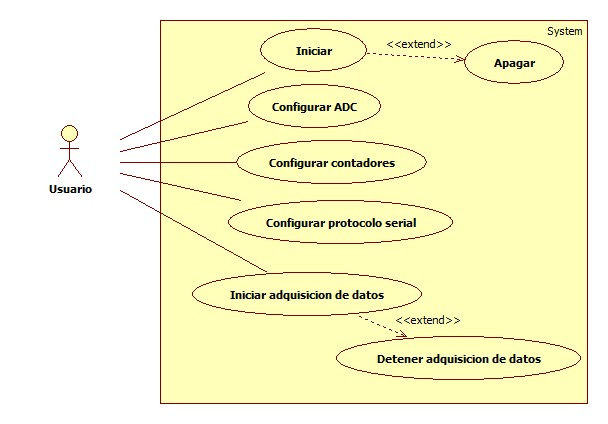
\includegraphics[width=0.80\textwidth, height = 9cm]{CasoUso1}
  \caption{Caso de uso 1}\label{fig:casouso1}
\end{figure}

\subsubsection{Diagramas de secuencia}
Los diagramas de secuencia modelan distintas interacciones entre los componentes de un sistema. En este caso, los dos componentes mas importantes del sistema son el usuario, y el programa principal que recibe las peticiones del usuario a traves de la interfaz grafica, y procesa los pedidos llamando a funciones de otros bloques del sistema. En el primer diagrama (figura \ref{fig:secuencia1}) se modelo una configuracion de un pin especifico para medir una entrada analogica. El programa principal, en este caso, debe llamar a funciones del bloque conversor para configurar el pedido del usuario. Luego, el usuario habilita el comienzo de conversion para que el sistema envie los datos ya digitales por interfaz serial.

\begin{figure}[h]
  \centering
  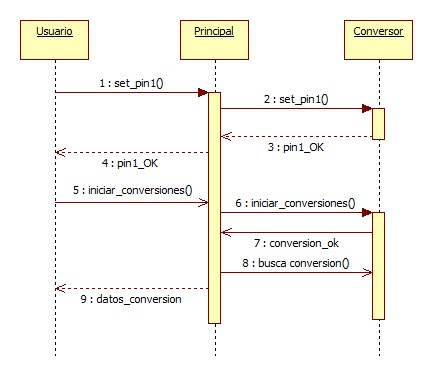
\includegraphics[width=0.50\textwidth, height = 7cm]{Secuencia1}
  \caption{Diagrama de secuencia 1}\label{fig:secuencia1}
\end{figure}

El diagrama en la figura \ref{fig:secuencia2} muestra una configuracion de un contador. En este sistema, los contadores se inician junto con el arranque mismo del sistema y desde ahi mismo comienzan a contar los eventos que ocurran en el pin que tienen asignado. Es por esto que lo unico que hay que hacer es consultar el valor en los registros asociados al contador para obtener la cuenta actual.

El diagrama \ref{fig:secuencia3} muestra una obtencion y un guardado de datos de configuracion en la memoria flash del microcontrolador. Los datos de configuracion son unicamente los pertenecientes al conversor analogico-digital.

\begin{figure}[h]
  \centering
  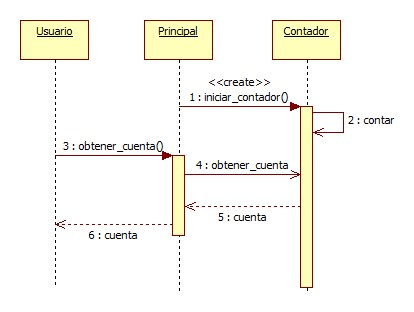
\includegraphics[width=0.50\textwidth, height = 7cm]{Secuencia2}
  \caption{Diagrama de secuencia 2}\label{fig:secuencia2}
\end{figure}


\begin{figure}[H]
  \centering
  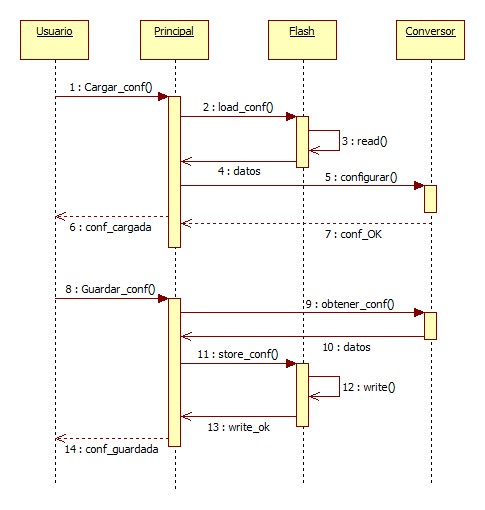
\includegraphics[width=0.60\textwidth, height = 8cm]{Secuencia3}
  \caption{Diagrama de secuencia 3}\label{fig:secuencia3}
\end{figure}

\section{Avances con respecto al dise�o de software}
En las primeras 100 horas no fue posible cubrir los requerimientos principales. Los avances obtenidos hasta hoy son los siguientes

\begin{itemize}
  \item Es posible configurar las entradas del ADC en modo single-ended y bipolar
  \item Es posible dar una ganancia de 2 a 128 para cada entrada del conversor
  \item Es posible contar eventos con dos contadores distintos
  \item Es posible modificar la tasa de envio de datos por UART para cada se�al convertida por separado
\end{itemize}

\section{Estructura del software}
El programa esta dividido en 6 modulos que en la mayoria de los casos corresponde a cada bloque en el que esta dividido el sistema, como se muestra en la figura \ref{fig:bloques1}

\subsection{Partes que conforman el software}
En este momento, el programa entero esta compuesto por 6 modulos. Un modulo principal y otros 5 que definen funciones segun los bloques que describen el comportamiento del sistema. El modulo principal ejecuta las funciones de los modulos secundarios.

\paragraph{}
\textbf{Modulos:}
\begin{itemize}
  \item Principal
  \item Conversor
  \item Contador
  \item Interrupciones
  \item Configurador
  \item Interfaz de Usuario
\end{itemize}

\subsubsection{Configurador}\label{sec:configuradorsw}
El configurador se encarga de inicializar todos los parametros necesarios que permiten la operatividad del resto de los modulos. Establece los valores correspondientes para todos los registros pertinentes y configura los puertos seleccionados en el modulo del conversor (Secci�n \ref{sec:conversorsw}) cuando se especifique por parte del usuario.
\subsubsection{Principal}
El modulo principal es la funcion main, inicializa todo el sistema usando funciones del configurador (Seccion \ref{sec:configuradorsw}) y hace el loop infinito que corre el sistema indefinidamente, obteniendo los comandos del usuario via la interfaz (Seccion \ref{secc:interfaz}).

\subsubsection{Conversor}\label{sec:conversorsw}
El modulo de conversion se encarga de la etapa de obtencion y procesado de las se�ales convertidas del ADC (Secci�n \ref{sec:adc}).

Las funciones de este modulo se encargan de que la obtencion de los datos se corresponda con la configuracion dada por el usuario. Es por esto que tiene funciones que se activan en la etapa de configuracion del sistema que preparan al mismo para una obtencion de datos conforme a los ajustes hechos por el usuario. Estos ajustes se realizan mediante las instrucciones MML mencionadas en la seccion \ref{secc:interfaz} y explicadas con detalle en el apendice \ref{ap:instrucciones}.


\subsubsection{Interfaz de usuario}\label{secc:interfaz}
En un principio, se comenzo con una interfaz de usuario pensada en forma de un menu principal. La idea era que un pueda acceder a todas las opciones de configuracion del sistema desde este menu, ingresando opciones por teclado y cambiando asi los parametros. La ventaja de este metodo es que los errores por parte del usuario se reducen significativamente, dado que no tiene otra opcion que elegir entre las opciones que muestra el menu. La desventaja es la complejidad que implica hacer un sistema altamente configurable con una interfaz de este tipo. Esta desventaja fue finalmente la que hizo que se cambiara la interfaz por completo, ya que luego de algunas semanas, las opciones de configuracion comenzaron a crecer y se hizo evidente que una interfaz de menu hacia la configuracion muy arduosa para el usuario y muy complicada de cambiar y hacer para el programador.Por lo que se cambio a un metodo con mas libertades para el usuario y menos complejidad para el programador.

La interfaz de usuario actual esta hecha con un lenguaje de especificacion denominado "Man Machine Languaje". MML es un lenguaje de especificacion que se usa tipicamente para estandarizar la interfaz de un sistema para el manejo del mismo desde una consola. Siguendo el paradigma de MML, lo que se hace es definir una serie de comandos que pueden aceptar una serie de argumentos. Con cada comando y sus argumentos se conforma una orden que ejecuta el procesador. De esta manera, se pueden lograr instrucciones simples que cambian distintos aspectos de la configuracion del sistema conforme a las intenciones del usuario. Una descripcion completa de las instrucciones hechas hasta el momento se encuentra en el apendice \ref{ap:instrucciones}. Con esto, es posible configurar todos los aspectos del sistema, sabiendo como operan todas las instrucciones y sus argumentos.

Este esquema de interfaz de usuario esta todavia en proceso. Hasta ahora, las instrucciones descriptas en el apendice \ref{ap:instrucciones} no cubre por completo todas las configuraciones que deberian poder hacerse teniendo en cuenta los requerimientos principales del sistema.


\subsubsection{Contador}
El modulo de contador contiene funciones que devuelven los valores de las cuentas actuales de los contadores en funcionamiento. Por una cuestion de simpleza, los contadores siempre estan activos, ya sea que se usen o no. Actualmente se cuenta con tres contadores de eventos. El microcontrolador tiene cuatro timers (Secci�n\ref{sec:contadores}) pero obligadamente uno de ellos debe ser utilizado por el modulo de la interfaz serial UART (Secci�n\ref{sec:serial}).

Cada contador utilizable tiene una funcion que simplemente se encarga de obtener el valor de la cuenta en su respectivo timer asociado. Las instrucciones definidas en MML(Seccion \ref{secc:interfaz}) descriptas en el apencice \ref{ap:instrucciones} incluyen las instrucciones GT0, GT1, y GT2, que se utilizan para la obtencion del valor de la cuenta actual.
%\begin{equation}\label{eq:area}
%  S = \pi r^2
%\end{equation}
%Uno puede referirse a ecuaciones as�: ver ecuaci�n (\ref{eq:area}).
%Tambi�n se pueden mencionar secciones de la misma forma: ver secci�n
%\ref{sec:nada}. O citar algo de la bibliograf�a: \cite{Cd94}.
\subsubsection{Interrupciones}
Este archivo define las rutinas de interrupcion para aquellas funcionalidades que se requiere que realicen interrupciones sobre el microcontrolador para condicionar el comportamiento del programa. Actualmente el conversor analogico-digital\ref{sec:adc} es el unico modulo que realiza interrupciones.


\clearpage
\appendix
\begin{appendices}
   \addappheadtotoc
   \appendixpage


\section{Instrucciones MML}\label{ap:instrucciones}

\subsection{SSE (Set Single Ended)}

\textbf{Formato:} SSE,[1]

\textbf{Descripcion:}
Establece el pin ingresado en modo single ended.

\textbf{Limitaciones:}
\begin{itemize}
  \item Un solo argumento
  \item El argumento es un byte par comprendido entre 0 y 7
\end{itemize}

\textbf{Ejemplo:}

SSE,4: Establece el pin 4 del ADC en modo single ended

\subsection{SDI (Set Diferencial)}

\textbf{Formato:} SDI,[1]

\textbf{Descripcion:}
Establece el pin ingresado y el pin siguiente a ese en numero en modo diferencial

\textbf{limitaciones:}
\begin{itemize}
  \item un solo argumento
  \item el argumento es un byte par comprendido entre 0 y 6
\end{itemize}

\textbf{ejemplo:}

SDI,2: setea los pines 2 y 3 en modo diferencial

\subsection{SGA (Set Ganancia)}

\textbf{Formato:} SGA,[1]

\textbf{descripcion:}
Establece la ganancia del ADC segun el argumento a la potencia de 2

\textbf{Limitaciones:}
\begin{itemize}
  \item Un solo argumento
  \item El argumento es un byte comprendido entre 0 y 7
\end{itemize}

\textbf{Ejemplo:}

SGA,3: Establece la ganancia en $2^{3} = 8$


\subsection{GT0 (Get Timer 0)}

\textbf{Formato:} GT0[0]

\textbf{Descripcion:}
Obtiene el valor actual de la cuenta de los eventos digitales monitoreados por timer0

\textbf{Limitaciones:}
\begin{itemize}
  \item No lleva argumentos


\end{itemize}\subsection{GT2 (Get Timer 2)}

\textbf{Formato:} GT2[0]

\textbf{descripcion:}
Obtiene el valor actual de la cuenta de los eventos digitales monitoreados por timer2

\textbf{Limitaciones:}
\begin{itemize}
  \item No lleva argumentos
\end{itemize}

\subsection{ST (Start)}

\textbf{Formato:} ST[0]

\textbf{Descripcion:}
Guarda los cambios, sale del modo de configuracion y comienza a correr el programa

\textbf{Limitaciones:}
\begin{itemize}
  \item No lleva argumentos
\end{itemize}

\end{appendices}
% Bibliograf�a.
%-----------------------------------------------------------------
\begin{thebibliography}{99}

\bibitem{bib:datasheet} Silicon Laboratories \emph{C8051F351/2/3} 8K ISP Flash MCU Family

\end{thebibliography}




\end{document} 